\chapter{Epithelium}
\begin{center}
``All models are wrong, but some are useful'' - G. Pox
\end{center}
\section{About Epithelium}
For my Master's Thesis I have implemented the Nagai-Honda Model for epithelial tissue development. My software is easy to install, takes up less than 50Mb, comes in parallel and non-parallel versions (Version 1.0.0, Version 1.0.1) and has very few dependencies (and they are likely already installed on mac and linux computers). 

My code allows users to specify all parameters of interest in a couple of well commented configuration files, can handle simulations of arbitrarily large size, and can generate beautiful animations and plots of epithelial tissue development as well as useful plots of various quantities which are of interest to the researcher. 

On top of all of this, the source code is highly modularized and allows for ambitious users to easily extend the code to meet their needs. For example, alternate numerical integrators can easily replace the existing one, new mesh generators can replace the square mesh I have developed, and all data is output in very simple formats( which users with scriting experience can transform to fit into the graphical utilities of their choice). In addition, the cell and vertex classes are well documented and can be extended to output new data, as users may need. What follow are a few graphs to give some flavor of what \emph{Epithelium} can do.

Mention how Chaste was a step in the right direction, but the dependencies are too many and the it is difficult to get started. Epithelium is lightwiehgt and the code is easy to read, a better introductory tool. 
\section{Sample Configuration Files}
\subsection{config.txt}
In this file, the user an specify some global properties about the mesh, and some important quantities for how the simulation will proceed. Most of the quantities are self explanatory. The dimension of the mesh is explained in the Code Design chapter of this paper. The swap length , upper bound, and Max Swaps parameters are used for performing random transformations to the mesh in the beginning of the simulation. The swap length is the edge length below which a swap is performed. The Max Swaps is the maximum nuber of random perturbations the code will make to the mesh. The upper bound is an integer which is upper bound of the range for a random number generator. The random swaps occur when a `1' is generated, and we choose random numbers from [1:upper bound].

OFF is the file format given to the plotting program geomview to plot the mesh. You can specify how often the code prints an image. It must be a multiple of ten, so if you want more closely spaced images you can just drop the maximum step size for the numerical integrator. The numerical integrator takes adaptively sized steps, and this will be discussed in more detail later. 

\begin{lstlisting}
13 # Dimension of mesh MUST BE ODD!!!!
1 # Plot the energy in the system? [1/0]
1 # Make a movie in the end? [1/0]
0.01 # Maximum step size
1000 # Number of iterations
10 # frequency of OFF file output. Must be a multiple 10!
.1 # delta minimum vertex separation.
1000 # Max swaps
1.5 # swap length
2 # upper bound random number generator
1 # Make a bar graph of cell sides? [1/0]
0 # Make a histogram of the areas? [1/0]
0 # Make a histogram of the perimeters? [1/0]
\end{lstlisting}
\subsection{parameters.hpp}
In this header the user can define some global parameter values for the cells in the mesh. Unfortunately, you must recompile every time a parameter is changed. This could be rewritten such that parameters are read in from a configuration file, but that is just not the way the code was developed. 
\begin{lstlisting}
const double beta = 0.1;
const double lambda = 0.1;
const double pi = 3.141592;
const double t_gamma = 1;
const double t_area = 14.0;
\end{lstlisting}
\subsection{changemesh.txt}
This file is a configuration file, and does not require you to recompile when you change it. You can fine tune the properties of the cells in the mesh with this file.
\begin{lstlisting}
# This file contains number of gamma changes, 
# followed by the number of area changes, 
# followed by the indices and new values
2 3
16 4.0
17 5.1
3 1.0
4 1.0
10 3.7
\end{lstlisting}
\section{Image Gallery}
This selection of graphs captures the properties of the mesh with various choices of parameter values. The target area for each cell was set to 4.0, unless otherwise specified. A couple of plots have outliers in the number of sides the cells have, or in the perimeters attained. This is due to the individual specification of cell properties for a handful of cells. In this way, the distribution of cell properties was more finely controlled. The images come in groups of four. There are two parameter studies per page. On the right you will see the equilibrium area and perimeter reached after applying the force, and the on the right you will see the equilibrium distribution of cell shapes along with a plot of the decreasing energy in the mesh as a function of time.

\section{Why \emph{Epithelium} is a good piece of software}
To close our discussion of \emph{Epithelium} I would like to discuss why it is a great piece of software for \emph{you}. \emph{GrowFlesh} has only a couple of dependencies which are likely already installed on you computer if you are interested in computational science. You will need a compiler supporting the C++11 standard, python2.7,  the matplotlib plotting library for python and the numpy python library. The only packages which will likely not be installed on your computer are the geomview geometric visualization software and the imagemagick image conversion program. Geomview and ImageMagick are free, and are such good programs that they have been around for more than 20 years. Of course, all of the animation, and plot information is outputed from this software in file formats that are easy to adapt to the user's choice of visualization software. The energy and histogram files are space separated lists and the mesh information is outputted in the OFF file format, which features a list of coordinates followed by a list of polygons which are defined counterclockwise as a list of vertex indices from the preceding list of vertices. A  sample mesh file is shown below to convince you of how simple this file format is, and to suggest that you could write a smal script to change this file to a different format that will be acceptable to your choice of visualization software.

\begin{lstlisting}
{appearance {+edge}
OFF 
# This is the OFF formate for a square. 
# We have the numVerts, numFaces, and a zero
# Then a list of vertex coordinates
# Then a list of faces described counterclockwise 
# by their vertices.
4 1 0
1 0 0
1 1 0
0 1 0
0 0 0
4 1 2 3 4
\end{lstlisting}

\begin{figure}[h]
\centering
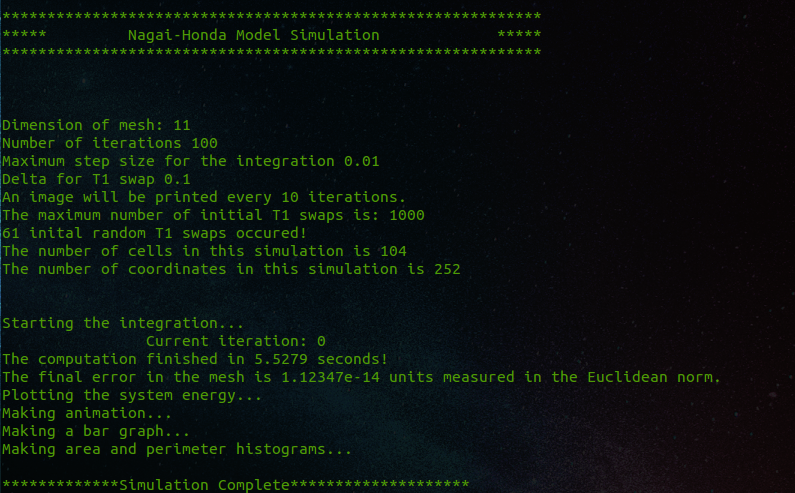
\includegraphics{../diagrams/screen.png}
\caption{A screenshot of the simulator}
\end{figure}
